% Results
The results of the raining process are presented in this chapter. We begin by first solving outlining the training network architecture and training process on simulated XANES in section \ref{sec:nn-sim-data}. Then, we discuss the work on expanding the model to make solid predictions on experimental data.

\section{Training with Simulation Data} \label{sec:nn-sim-data}
The 1000 simulated XANES spectra were first loaded into a Pandas dataframe \cite{pandas-1} \cite{pandas-2} of shape $ 1000\times82 $. Each of the 82 columns represents a discrete energy value, and each row represents the absorption for a given spectrum at those energies. The dataset was split into training and testing groups according to an 80-20 random split, respectively. All absorption columns were then scaled via the standard scalar (\ref{z-score}) and the training labels scaled via a min-max scaler (\ref{eqn:min-max-scaler}). First, the model was trained to predict four descriptors: the mean-squared-displacement (MSD), the mean bond length distance, the standard deviation of the bond length distributions, and the skew of the bond length distribution. Note that the standard deviation is the same as the square root of the MSD. This feature was only included preliminarily in order to better understand the correlation in the network's predictions. 

\bgroup
\def\arraystretch{1.5}%  1 is the default, change whatever you need
\begin{table}[h!]
    \centering
    \begin{tabular}{|l|l|l|}
    \hline
    Layer  Type    & Output Shape  & Number of Parameters \\ \hline
    Normalization  & (None, 82)    & 165                  \\ \hline
    Dense          & (None, 128)   & 10,624               \\ \hline
    Dense          & (None, 128)   & 16,512               \\ \hline
    Dense          & (None, 512)   & 25,088               \\ \hline
    Reshape        & (None, 8, 64) & 0                    \\ \hline
    1D-Convolution & (None, 6, 32) & 6,176                \\ \hline
    Dropout        & (None, 6, 32) & 0                    \\ \hline
    1D-Max-Pooling & (None, 3, 32) & 0                    \\ \hline
    Flatten        & (None, 96)    & 0                    \\ \hline
    Dense          & (None, 128)   & 12,416               \\ \hline
    Dense          & (None, 48)    & 6,192                \\ \hline
    Dense          & (None, 512)   & 25,088               \\ \hline
    Flatten        & (None, 512)   & 0                    \\ \hline
    Dense          & (None, 4)     & 513                  \\ \hline
    \end{tabular}
    \caption[NN-Architecture Optimized for Simulations]{The model architecture for the network trained entirely on simulation data (which performed poorly on experimental data) relies primarily on affine (Dense) and convolutional layers. The model includes 108,966 total parameters, with 108,801 of those being trainable.}
    \label{tb:nn-arch-sims}
\end{table}
\egroup


\begin{figure}
    \centering
    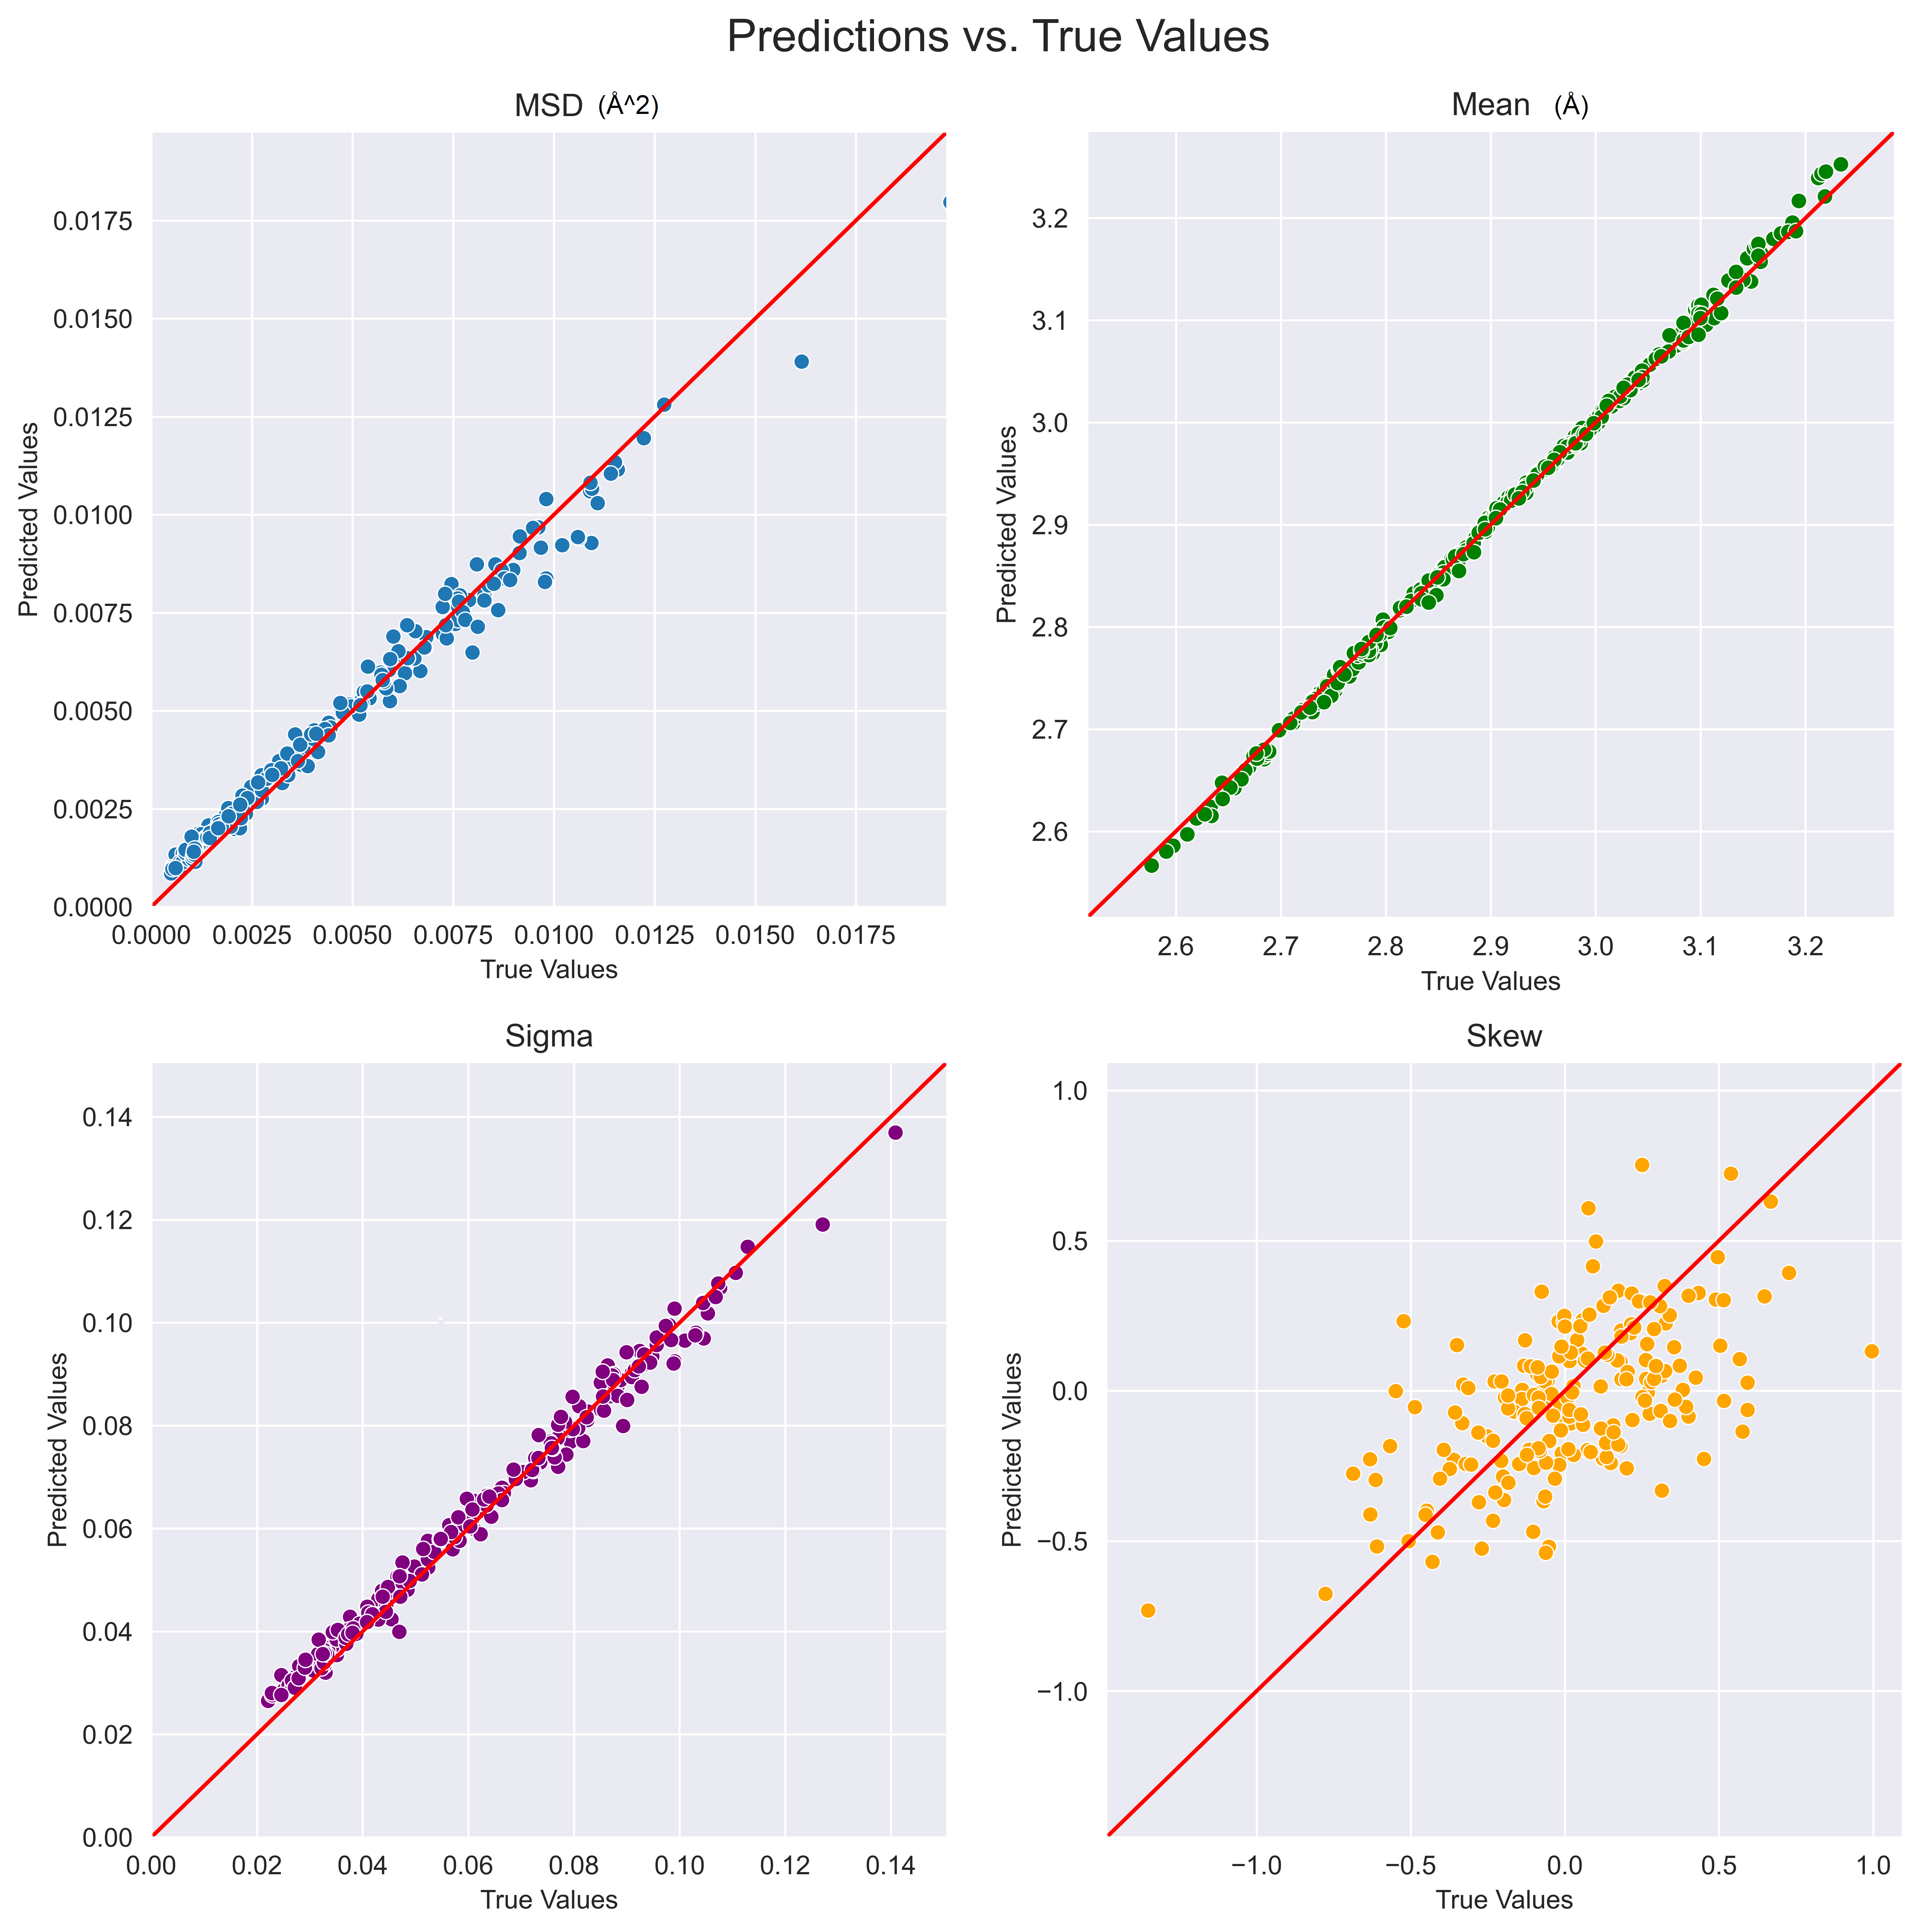
\includegraphics[width=\linewidth]{Chapters/Figures/pa_train-test-fixed.png}
    \caption{One configuration of the trained neural network includes four output nodes: MSD, Sigma, Mean, and Kurtosis. Sigma is just the square root of the MSD and was included during training to confirm the patterns recognized by the network. Each point in each subplot represents a FEFF simulated spectrum in the test set. For each spectrum, the y-axis represents the MSD value predicted by the NN, and the x-axis represents the true MSD (label) for that spectrum. Hence, points on the $ y=x $ red line are perfect predictions.}
    \label{fig:train-test-split-all4}
\end{figure}

\section{Experimental Data} \label{ch:results}

Training the neural network entirely on simulation data and then making predictions on experimental data is unlikely to provide quality results. Using the trained network from Table (\ref{tb:nn-arch-sims}) that predicted the test set values in Figure \ref{fig:train-test-split-all4}, we predicted the MSD values from two experimental spectra. On the unpublished IMASC data, the network predicted an MSD of $0.0003724~\AA^2$ instead of the EXAFS equation fitted value of ${\sigma^2=0.0102(8)~\AA^2}$. This poor prediction suggests the network considers the experimental spectrum to look most similar to the lowest disorder FEFF spectra; the model is not generalizing to understand the disorder encoded in the spectral shape.


\begin{figure}
    \centering
    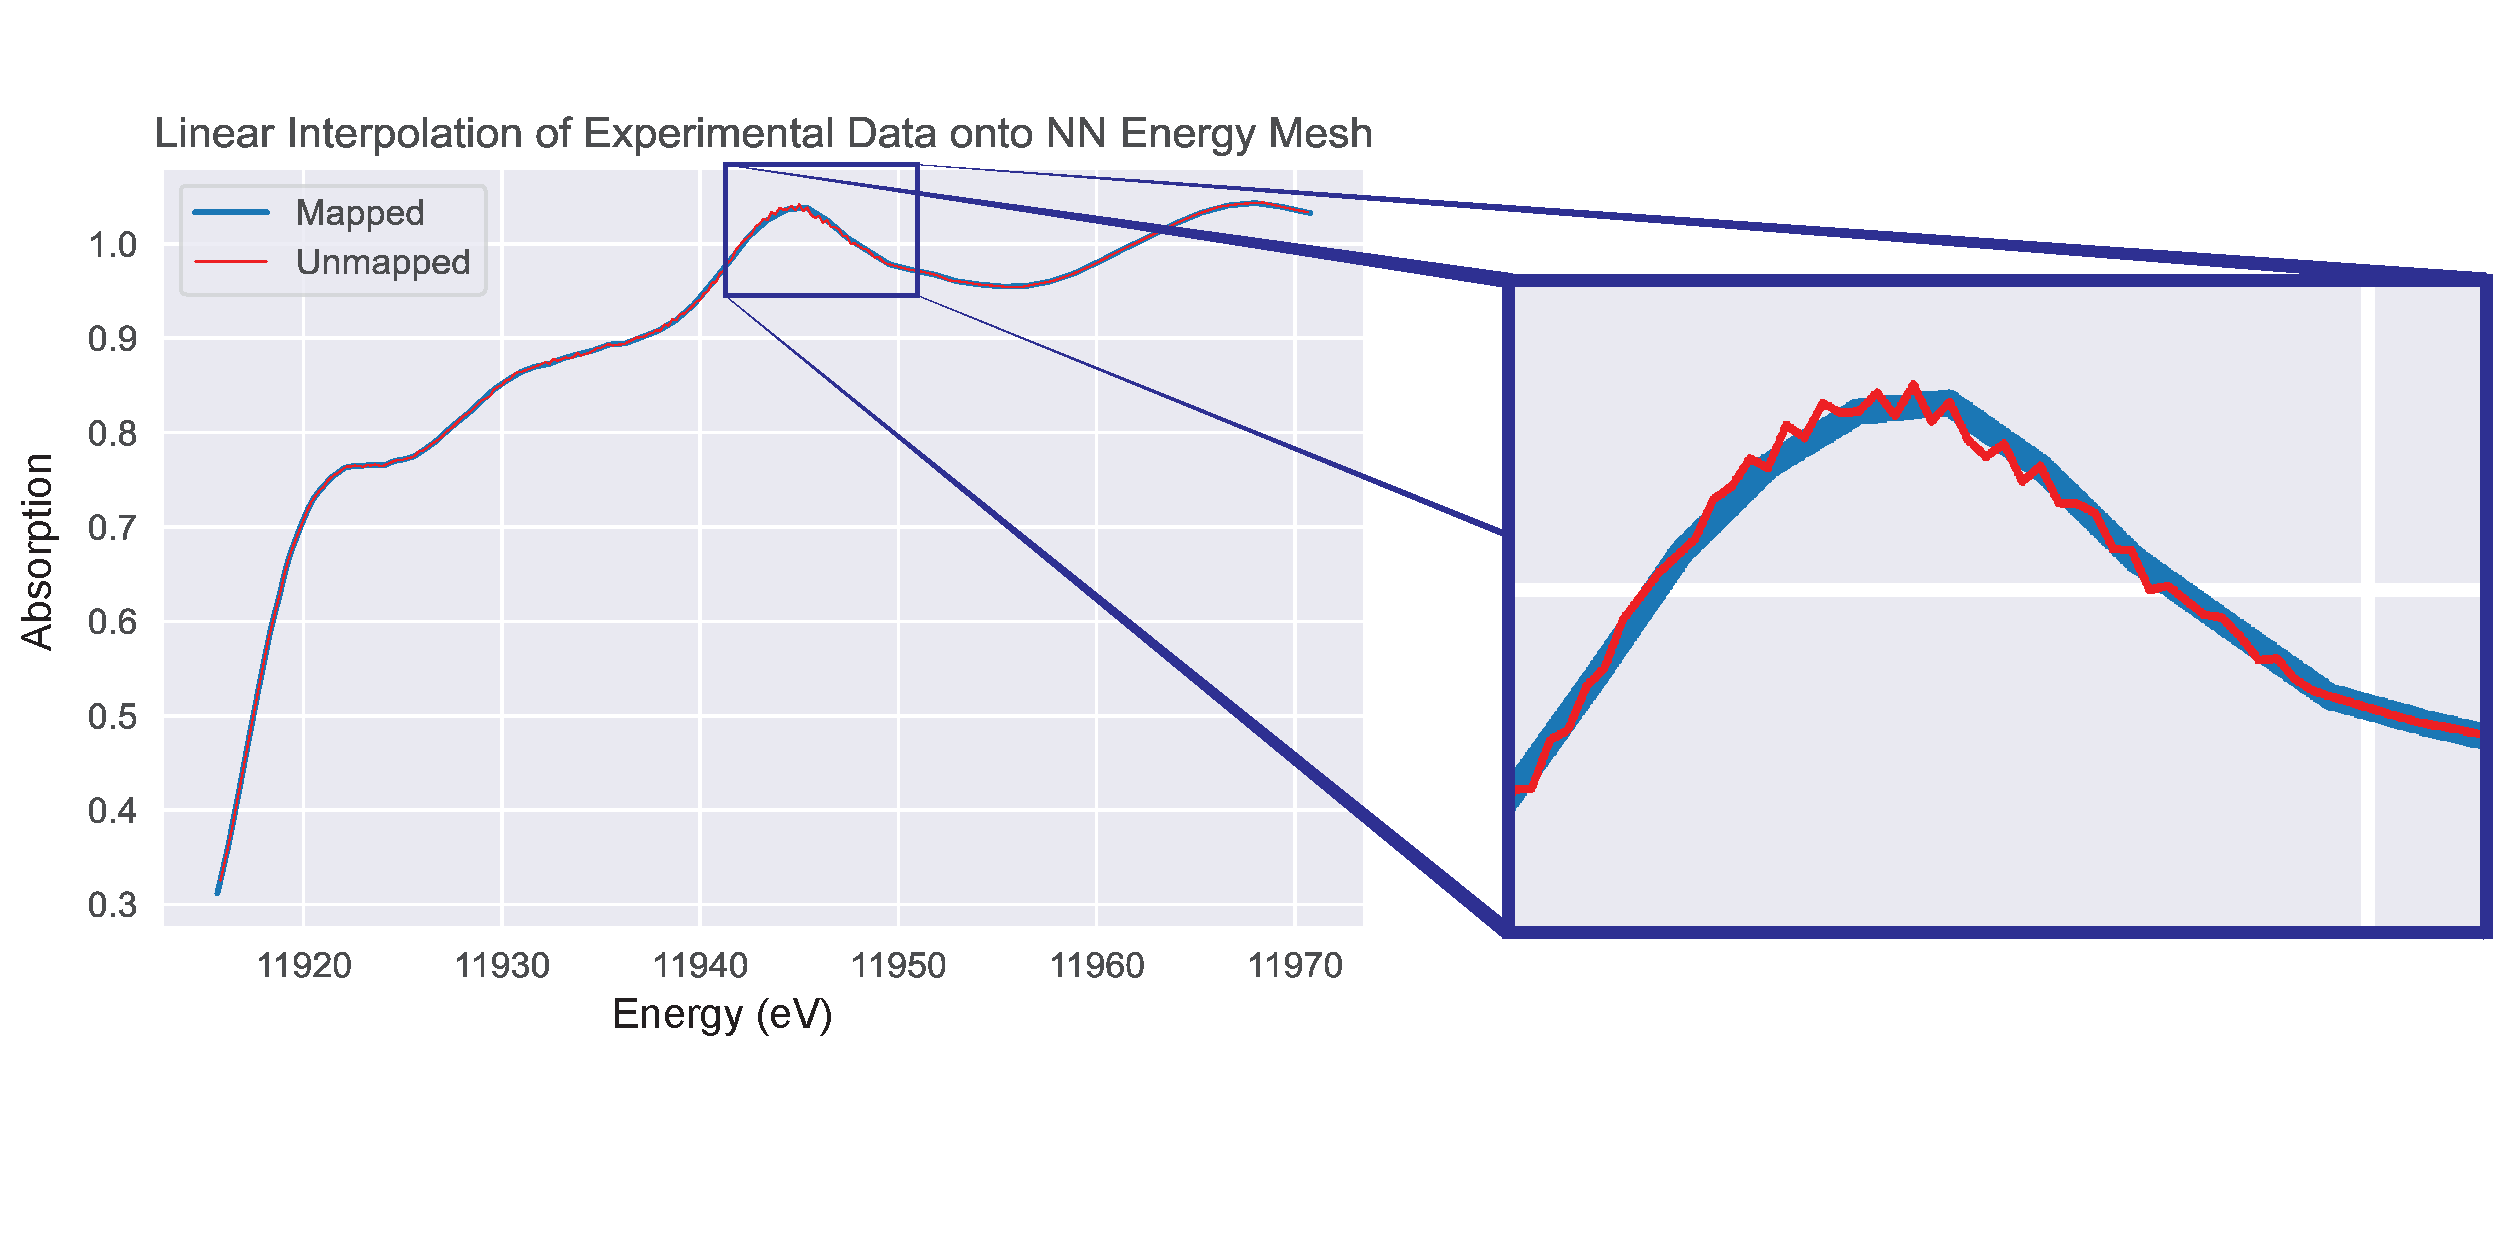
\includegraphics[width=\linewidth]{Chapters/Figures/quality-of-interpolation-skinny.pdf}
    \caption[Experimental Data Interpolation]{The experimental data is measured as a function of different energy values than the ones on which the neural network is trained. Consequently, the experimental spectrum must be mapped onto the proper energy mesh via linear interpolation.}
    \label{fig:interpolation-skinny}
\end{figure}

\subsection{Data Augmentation}
While there is ample data for training and predicting on only simulation data, we only have two experimental spectra. In order to create more training and testing data for the neural network, two types of data augmentation were utilized: horizontal spectral shifting and Gaussian noise inclusion. While the motivation for utilizing data augmentation is to expand the size of the experimental training and testing set, the neural network must be trained to recognize the augmentation types prior to training or testing on the experimental data. As such, both the FEFF simulated dataset and experimental dataset are augmented.

Noise is artificially injected into the spectra by randomly shifting each absorption coefficient vertically. The shifted value for each energy level is selected from a Gaussian distribution with standard deviation $ \sigma=0.01 $. An exaggerated example of the injected noise is shown in Figure \ref{fig:data-aug-gauss-noise}.

\begin{figure}[h!]
    \centering
    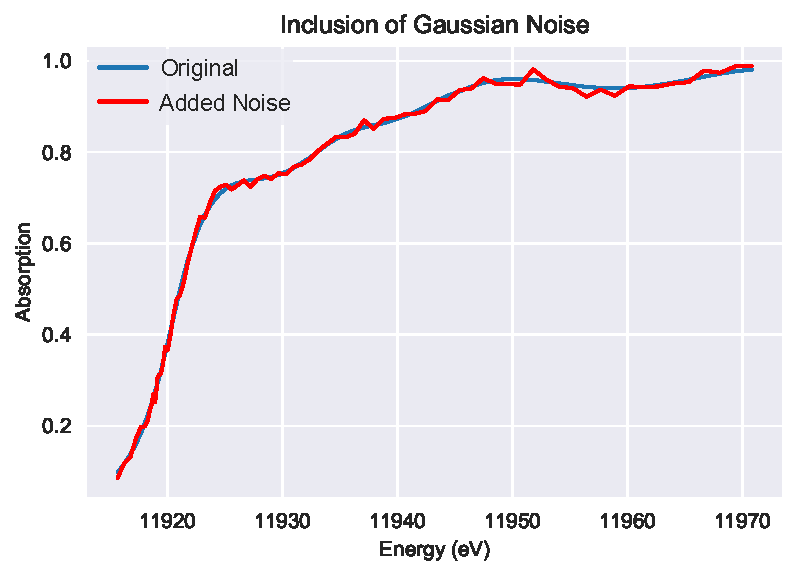
\includegraphics[width=.75\linewidth]{Chapters/Figures/gaussian-noise-data-aug.pdf}
    \caption[Data Augmentation: Gaussian Noise]{Gaussian noise is added to the spectra to increase the variance of the training data. This helps the network to learn the low-level features of the spectra and ignore artifacts not caused by the structural disorder. For demonstration purposes, the scale of the noise in this figure has been increased beyond what was used in training.}
    \label{fig:data-aug-gauss-noise}
\end{figure}

The second form of data augmentation utilizes horizontal shifts. While this is common for signal processing and time series analysis, the inclusion here is more controversial. In XAFS, the edge location is dependent on the oxidation/reduction state of the species. Shifting the horizontal location is akin to shifting the species of the model; however, the neural network is not being tasked to determine the oxidation state of the sample. Instead, the model is only tasked with predicting the mean-squared-displacement of the nanoparticle's bond lengths. The theory is that the disorder information is encoded in the  

\begin{figure}[h!]
    \centering
    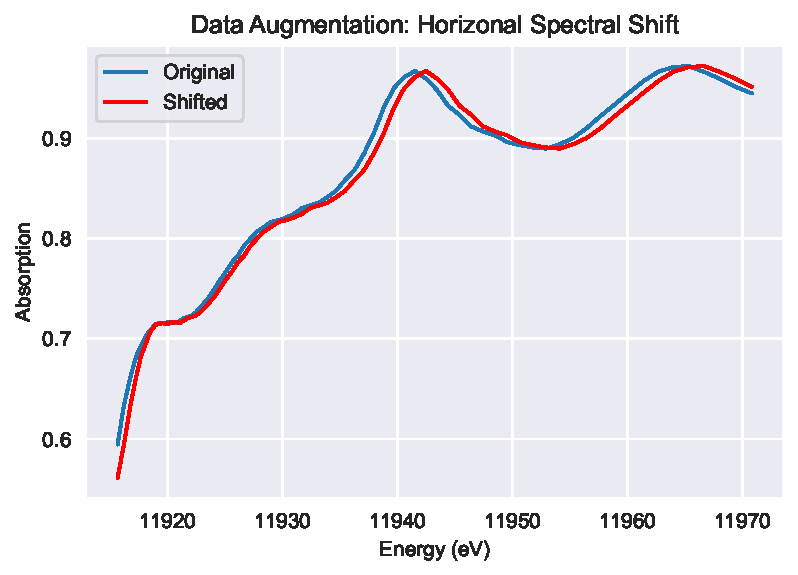
\includegraphics[width=.75\linewidth]{Chapters/Figures/data-aug-shift-pt75wieght.pdf}
    \caption[Data Augmentation: Horizontal Shift]{In order to train the network to predict disorder from the overall shape of the spectra---as opposed to fixating on the edge location---we introduce horizontal-shift as a data augmentation technique.}
    \label{fig:data-aug-hor}
\end{figure}

\subsection{Transfer Learning}
In building the transfer learning model, we opted to begin with a new network architecture, which can be found in Table (\ref{tab:meta-1}). We hypothesized that applying convolutional layers before any affine layers may lead to a more consistent prediction between simulation and experimental spectra.

\begin{figure}
    \centering
    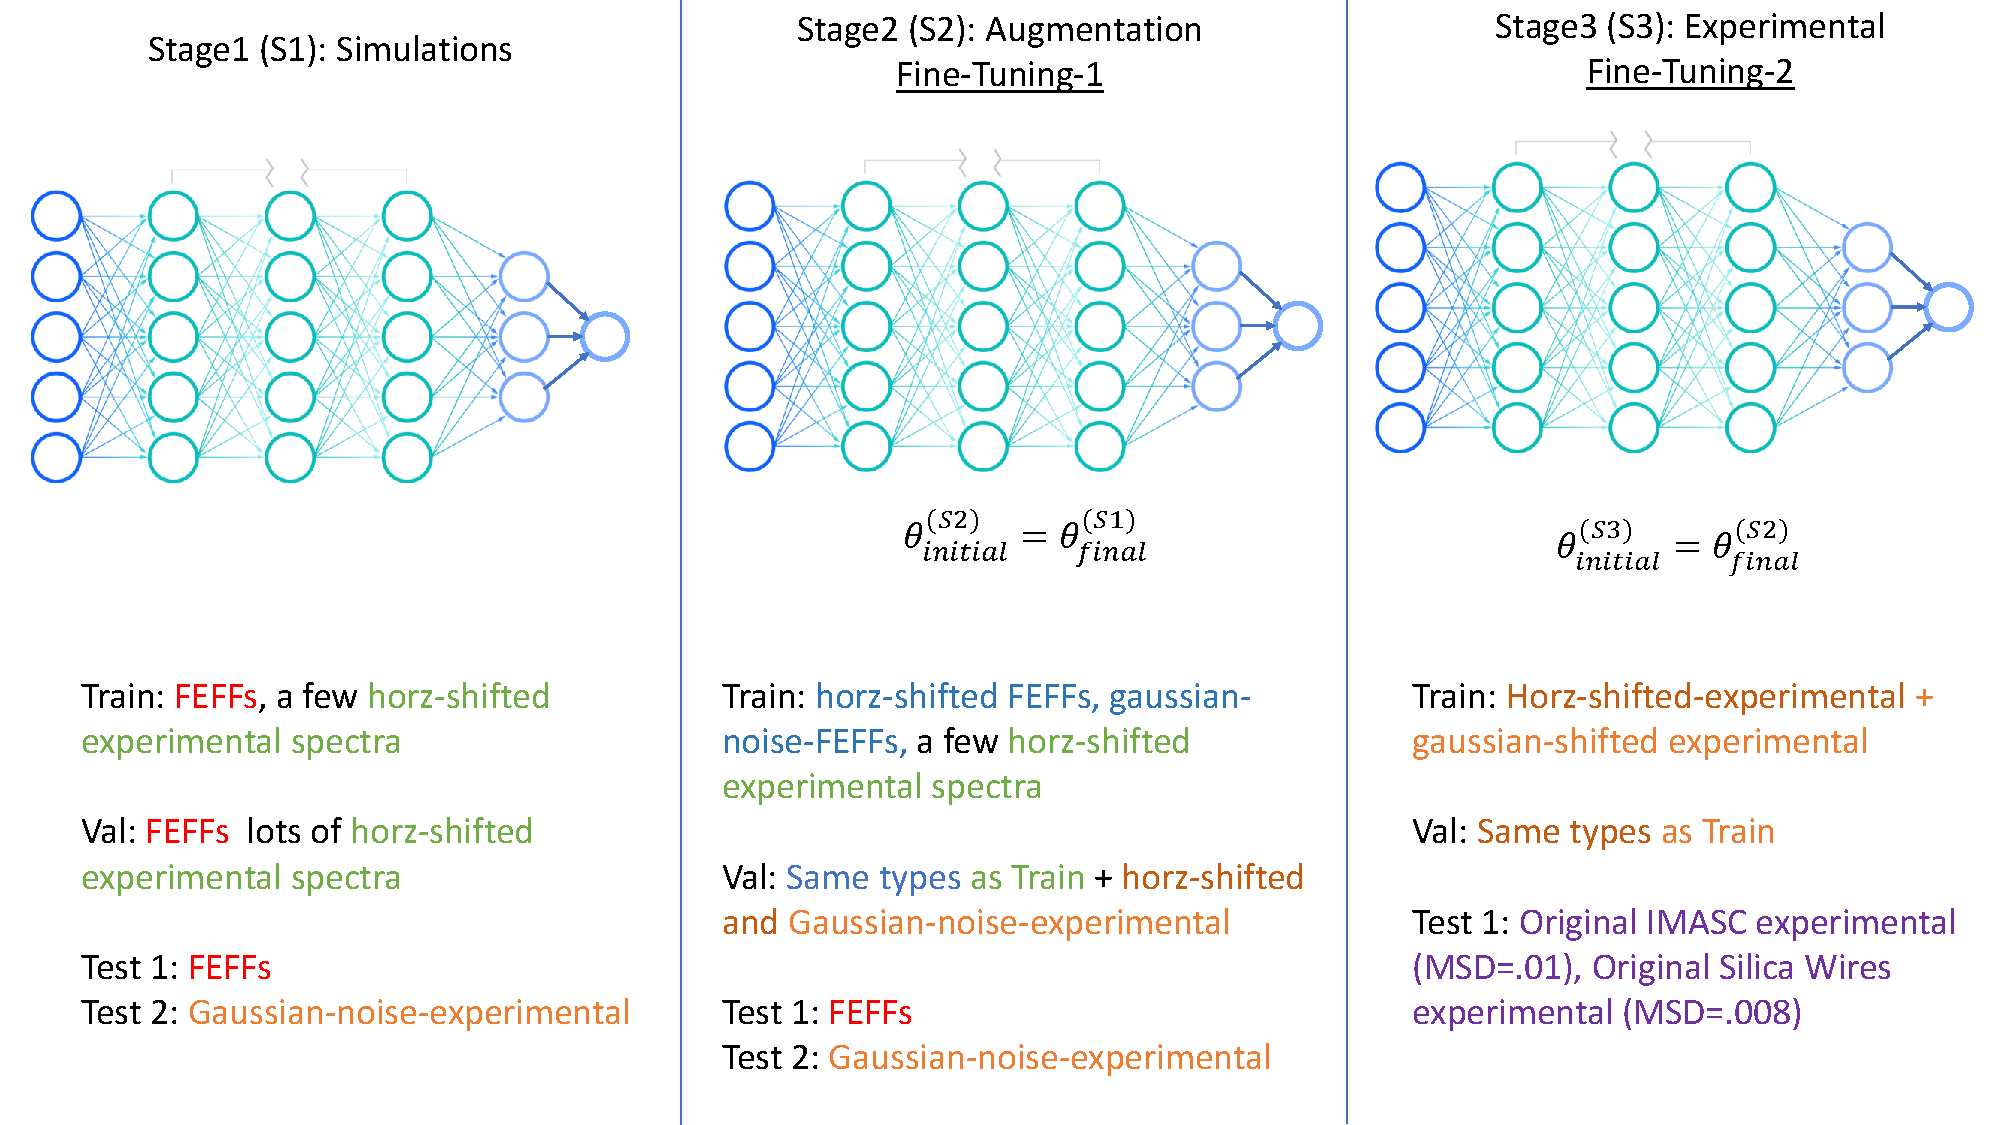
\includegraphics[width=\linewidth]{Chapters/Figures/transfer-learning-breakdown.pdf}
    \caption[Transfer Learning Process]{Caption here}
    \label{fig:transfer-learning-databreakdown}
\end{figure}

\bgroup
\def\arraystretch{1.5}
\begin{table}[]
    \centering
        \begin{tabular}{|l|l|l|l|}
        \hline
        \multicolumn{1}{|c|}{\textbf{Name}} & \multicolumn{1}{c|}{\textbf{Type}} & \multicolumn{1}{c|}{\textbf{\# Parameters}} & \multicolumn{1}{c|}{\textbf{Output Shape}} \\ \hline
        normalization\_input                & InputLayer                         & 0                                           &                                            \\ \hline
        normalization                       & Normalization                      & 165                                         & None, 82                                   \\ \hline
        reshape                             & Reshape                            & 0                                           & None, 82, 1                                \\ \hline
        conv1                               & Conv1D                             & 128                                         & None, 82, 32                               \\ \hline
        max\_pooling1d                      & MaxPooling1D                       & 0                                           & None, 41, 32                               \\ \hline
        conv2                               & Conv1D                             & 3104                                        & None, 39, 32                               \\ \hline
        max\_pooling1d\_1                   & MaxPooling1D                       & 0                                           & None, 19, 32                               \\ \hline
        flatten                             & Flatten                            & 0                                           & None, 608                                  \\ \hline
        dense1                               & Dense                              & 58464                                       & None, 96                                   \\ \hline
        dout                                & DropOut                            & 0                                           & None, 96                                   \\ \hline
        dense2                              & Dense                              & 30264                                       & None, 312                                  \\ \hline
        output                              & Dense                              & 313                                         & None, 1                                    \\ \hline
    \end{tabular}
    \caption{A new network architecture was constructed for the transfer learning process. The new network only has one output node, representing the MSD of the input spectrum.}
    \label{tab:meta-1}
\end{table}
\egroup

Our approach to succesfully applying transfer learning involves two stages of fine-tuning. First, we primarily  train the model on FEFF simulated spectra, selecting an architecture and hyperparameters which are likely to be compatible with fine-tuning. We achieve this by weighting the validation set heavily (around $ 10\% $) with augmented experimental spectra and choosing a model which performs as well predicting unseen data-augmented experimental spectra as it does predicting unseen simulated FEFF spectra. The training loss curves and selection process can be found in Figure \ref{fig:meta-1-sweep-loss}. One concern with this approach is that we are injecting biases into out model selection; however, we take this into account through utilization of a third, unseen test set, and the fact that the model does not update its parameters based on its predictions on the validation set. When training a model in machine learning, the parameters are continuously update until a minimum is reached in the loss function. While the loss function will have a global minimum, it also contains local minima, some of which will be more agnostic to the differences in experimental spectra and be better candidates for transfer learning. In this first stage of learning, the intention is to teach the model to find broad predictive features from the simulation set, while selecting a model at a local minimum which is likely to be a good transfer-learning candidate. 


\begin{figure}
    \centering
    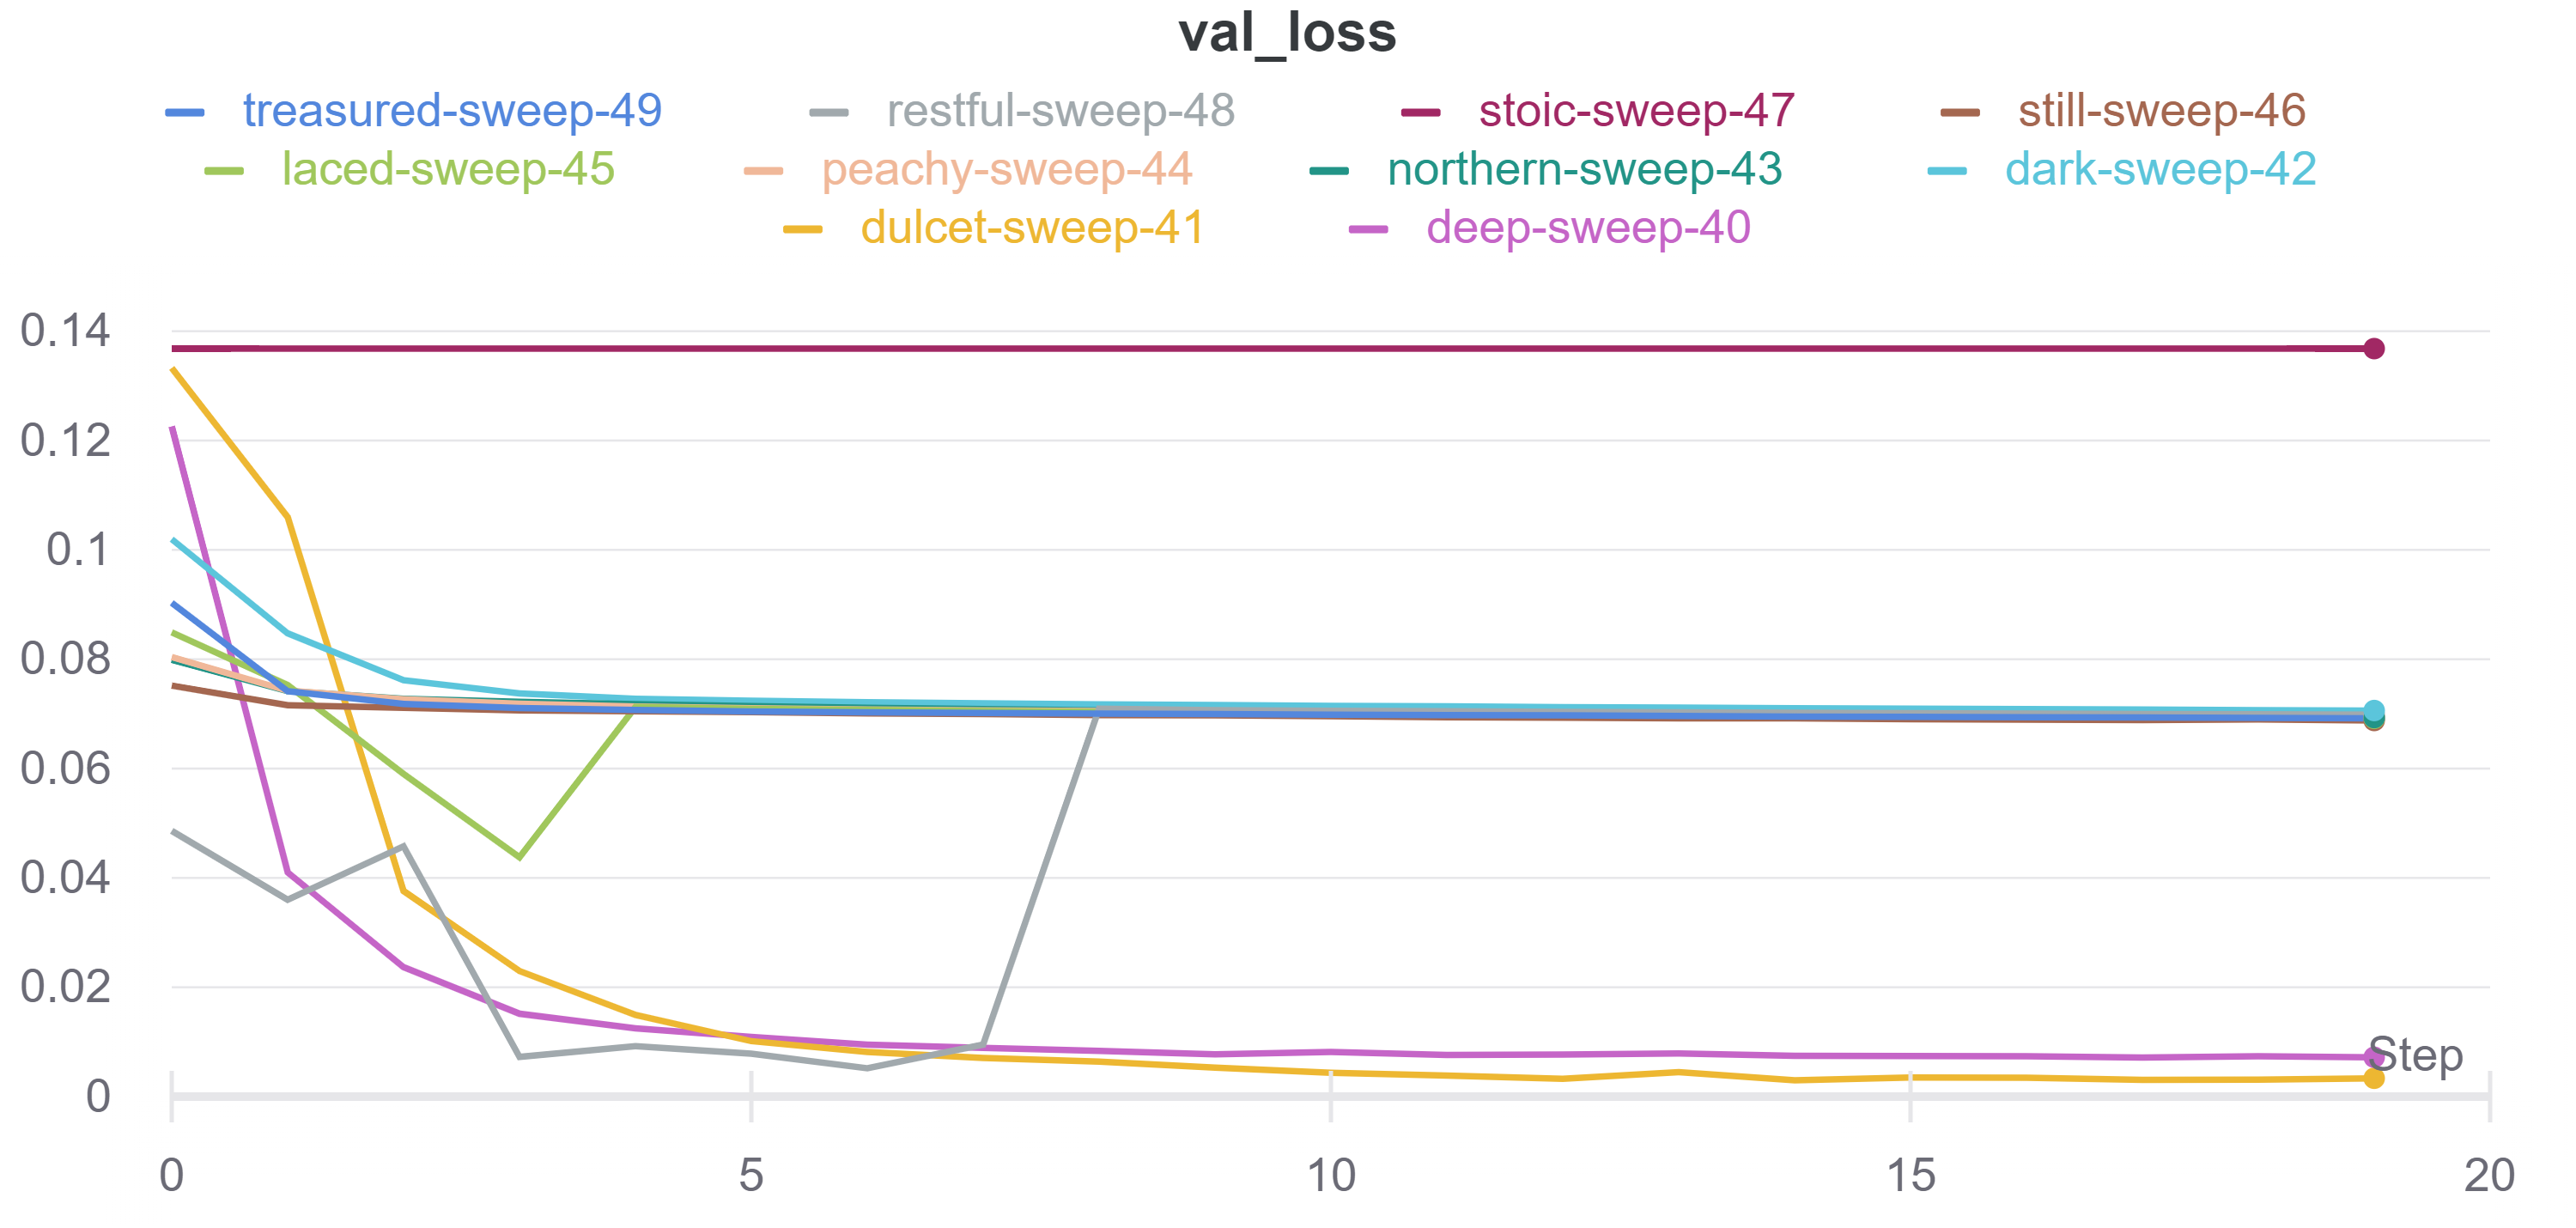
\includegraphics[width=\linewidth]{Chapters/Figures/10-sweep.png}
    \label{fig:meta-1-sweep-loss}
    \caption[Hyperpamater Sweep 1]{The validation loss (mean-squared-error) for 10 out of the 50 hyperparameter combinations searched in this sweep are plotted above. Most hyperparameters result in a loss curve stabilizing around 0.08, which is significantly higher than the training loss (not shown) that stabilized around 0.01. A few of the validation loss curves, instead, stabilized around 0.01 (dulcet-sweep-41 and deep-sweep-40). Because the validation set is heavily weighted with augmented experimental spectra, these two spectra are likely to be good candidates for transfer learning onto experimental data.}
\end{figure}

The next stage of transfer learning seeks to teach the model to ignore noise and focus on the broader shape of the spectrum. We achieve this by freezing the early stages of the model and retraining the later parameters on a new dataset comprised primarily entrirely of data-augmented spectra. Often, models are trained with the augmented dataset in the initial stage, which helps act as a form of regularization. In the case of transfer learning, however, applying this regularization so early on in the process may lead to undesirablr local minima for which transfer learning onto the experimental dataset would be impossible. By applying an initial stage of fine-tuning to a well-tuned base-model, we increase the likelyhood of a succesful second fine-tuning stage.

The last stage of the fine-tuning process is to freeze even more layers and reduce the learning rate, then train the model using all of the data-augmented experimental spectra. If the process is sucesful, the model will have learned to predict the MSD and ignore horizontal and gaussian noise in the spectra from the first stage. In this way, we have increased the number of possibly training samples to use for the final fine-tuning stage from one to many, and allowed us to withhold both of the un-altered experimental spectra from the training process and use them to evaluate the success of the transfer learning process. A visualization and specific breakdown of which data is allocated into each stage of the training process can be found in Figure \ref{fig:transfer-learning-databreakdown}.

\begin{figure}
    \centering
    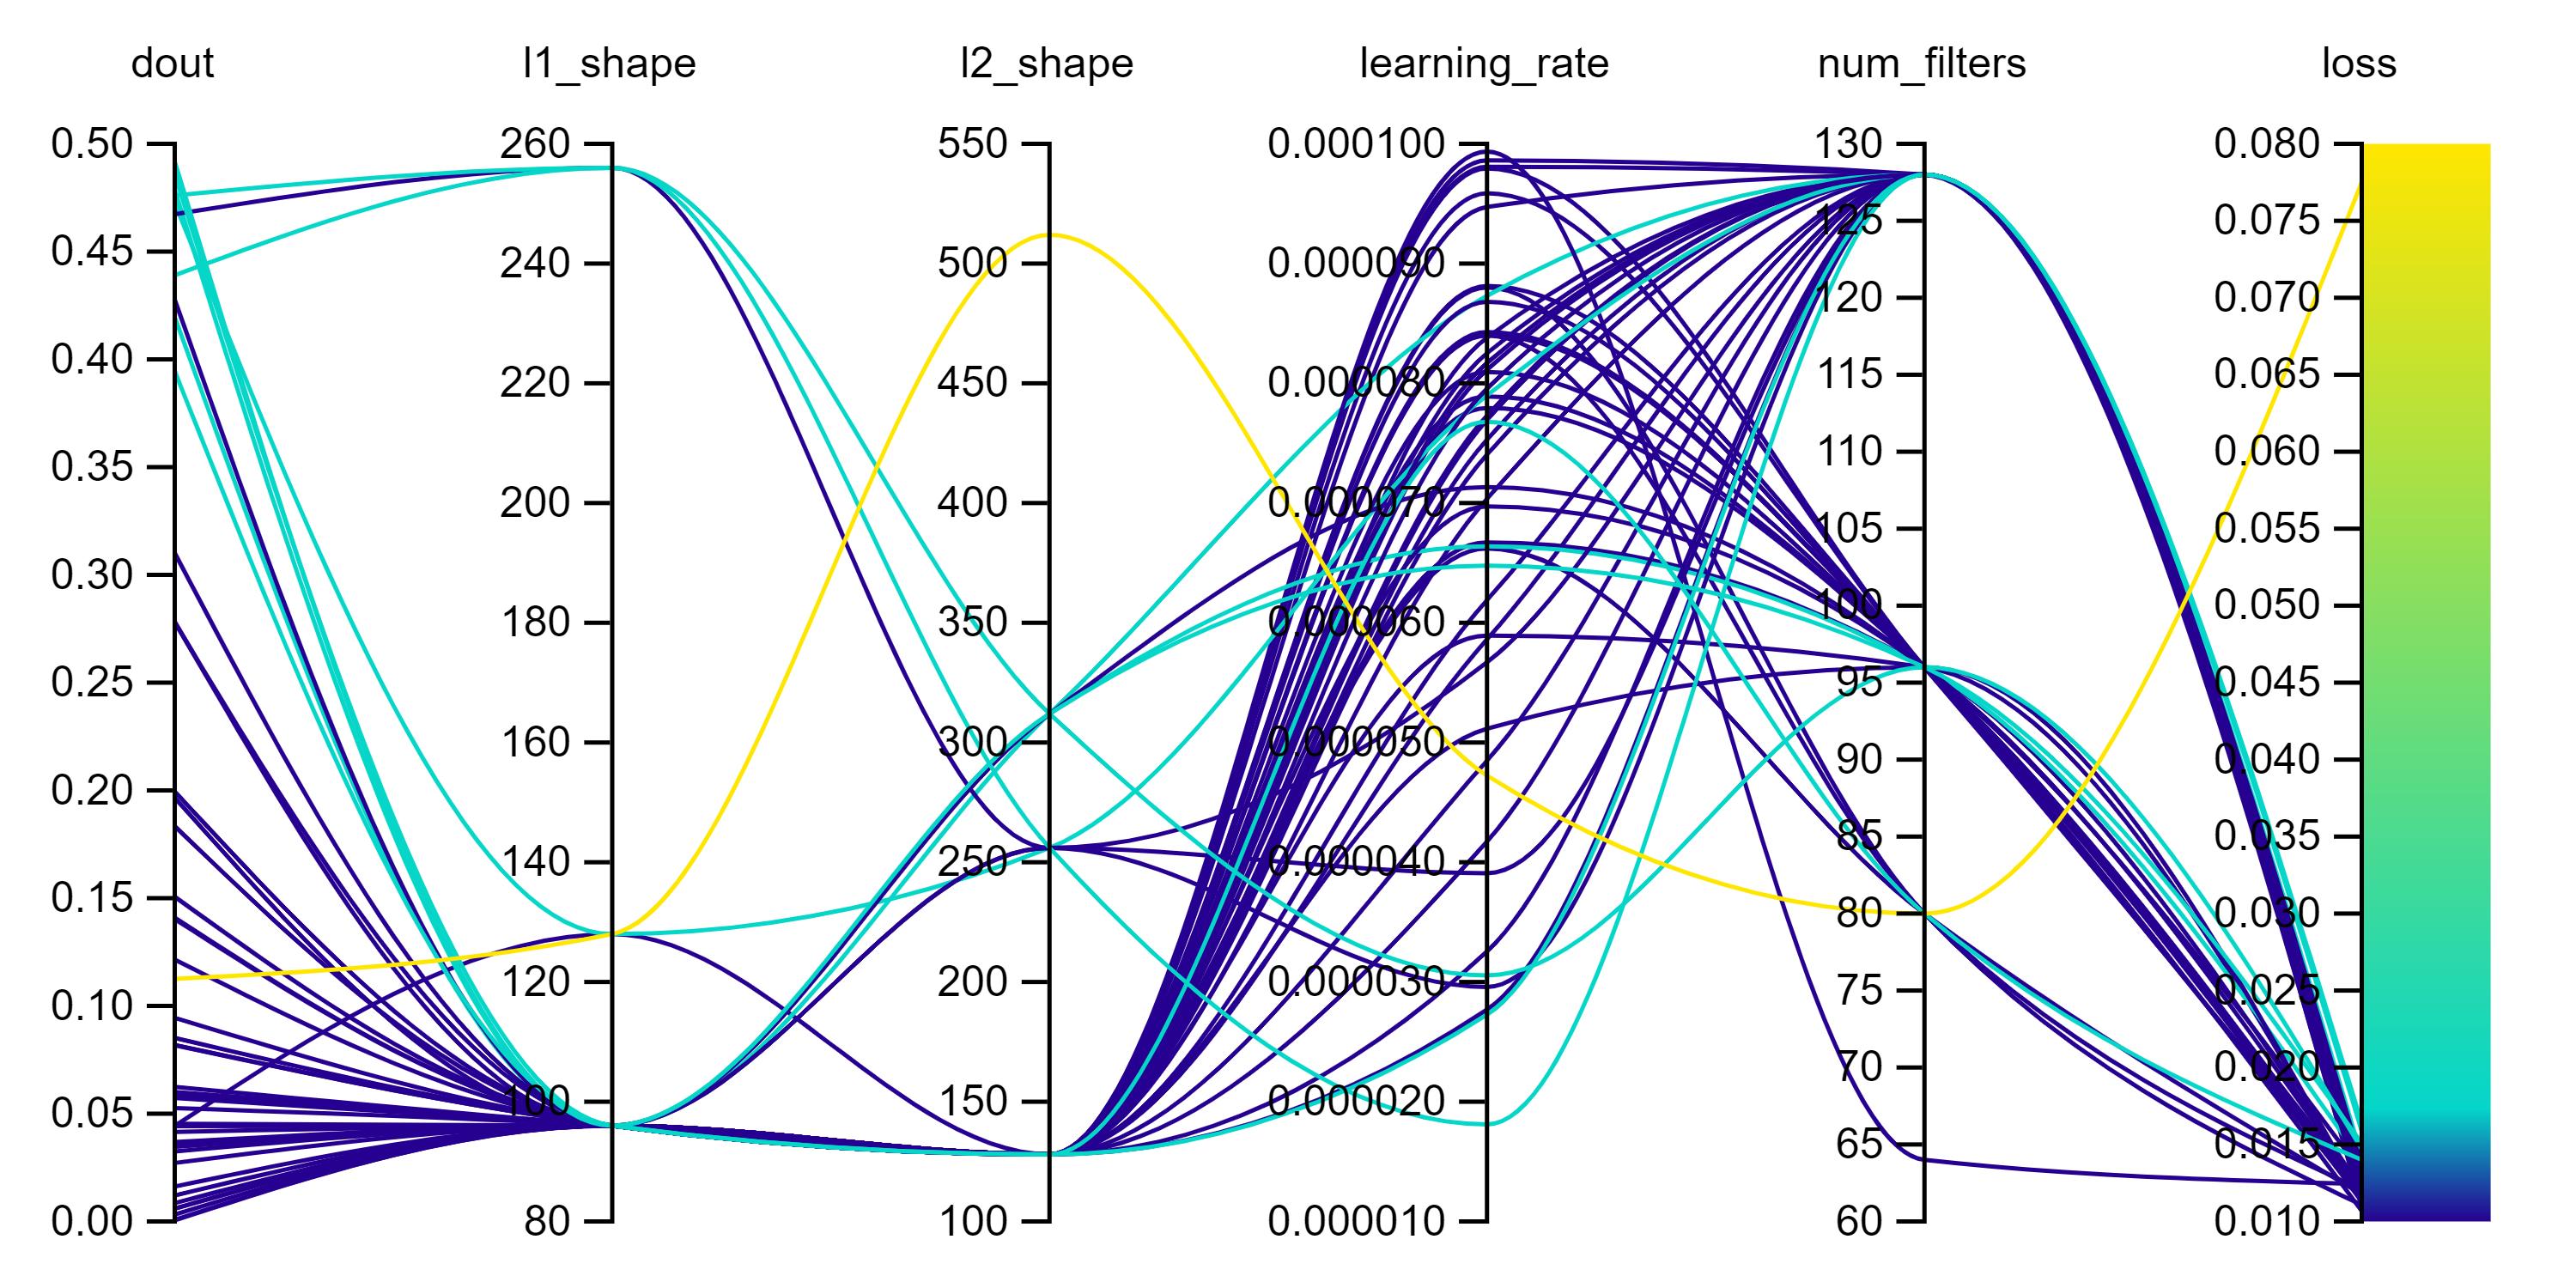
\includegraphics[width=\linewidth]{Chapters/Figures/new-hyperparameter-sweep-meta-1.png}
    \label{fig:meta-1-sweep-params}
    \caption[Hyperpamater Sweep 1]{The hyperparameters are obtained through a ``sweep,'' where the entire training process (20 epochs) is repeated with different hyperparameters each time. The hyperparameter training process and figure generation was conducted with the aid of \cite{wandb}.}
\end{figure}





\begin{figure}
    \centering
    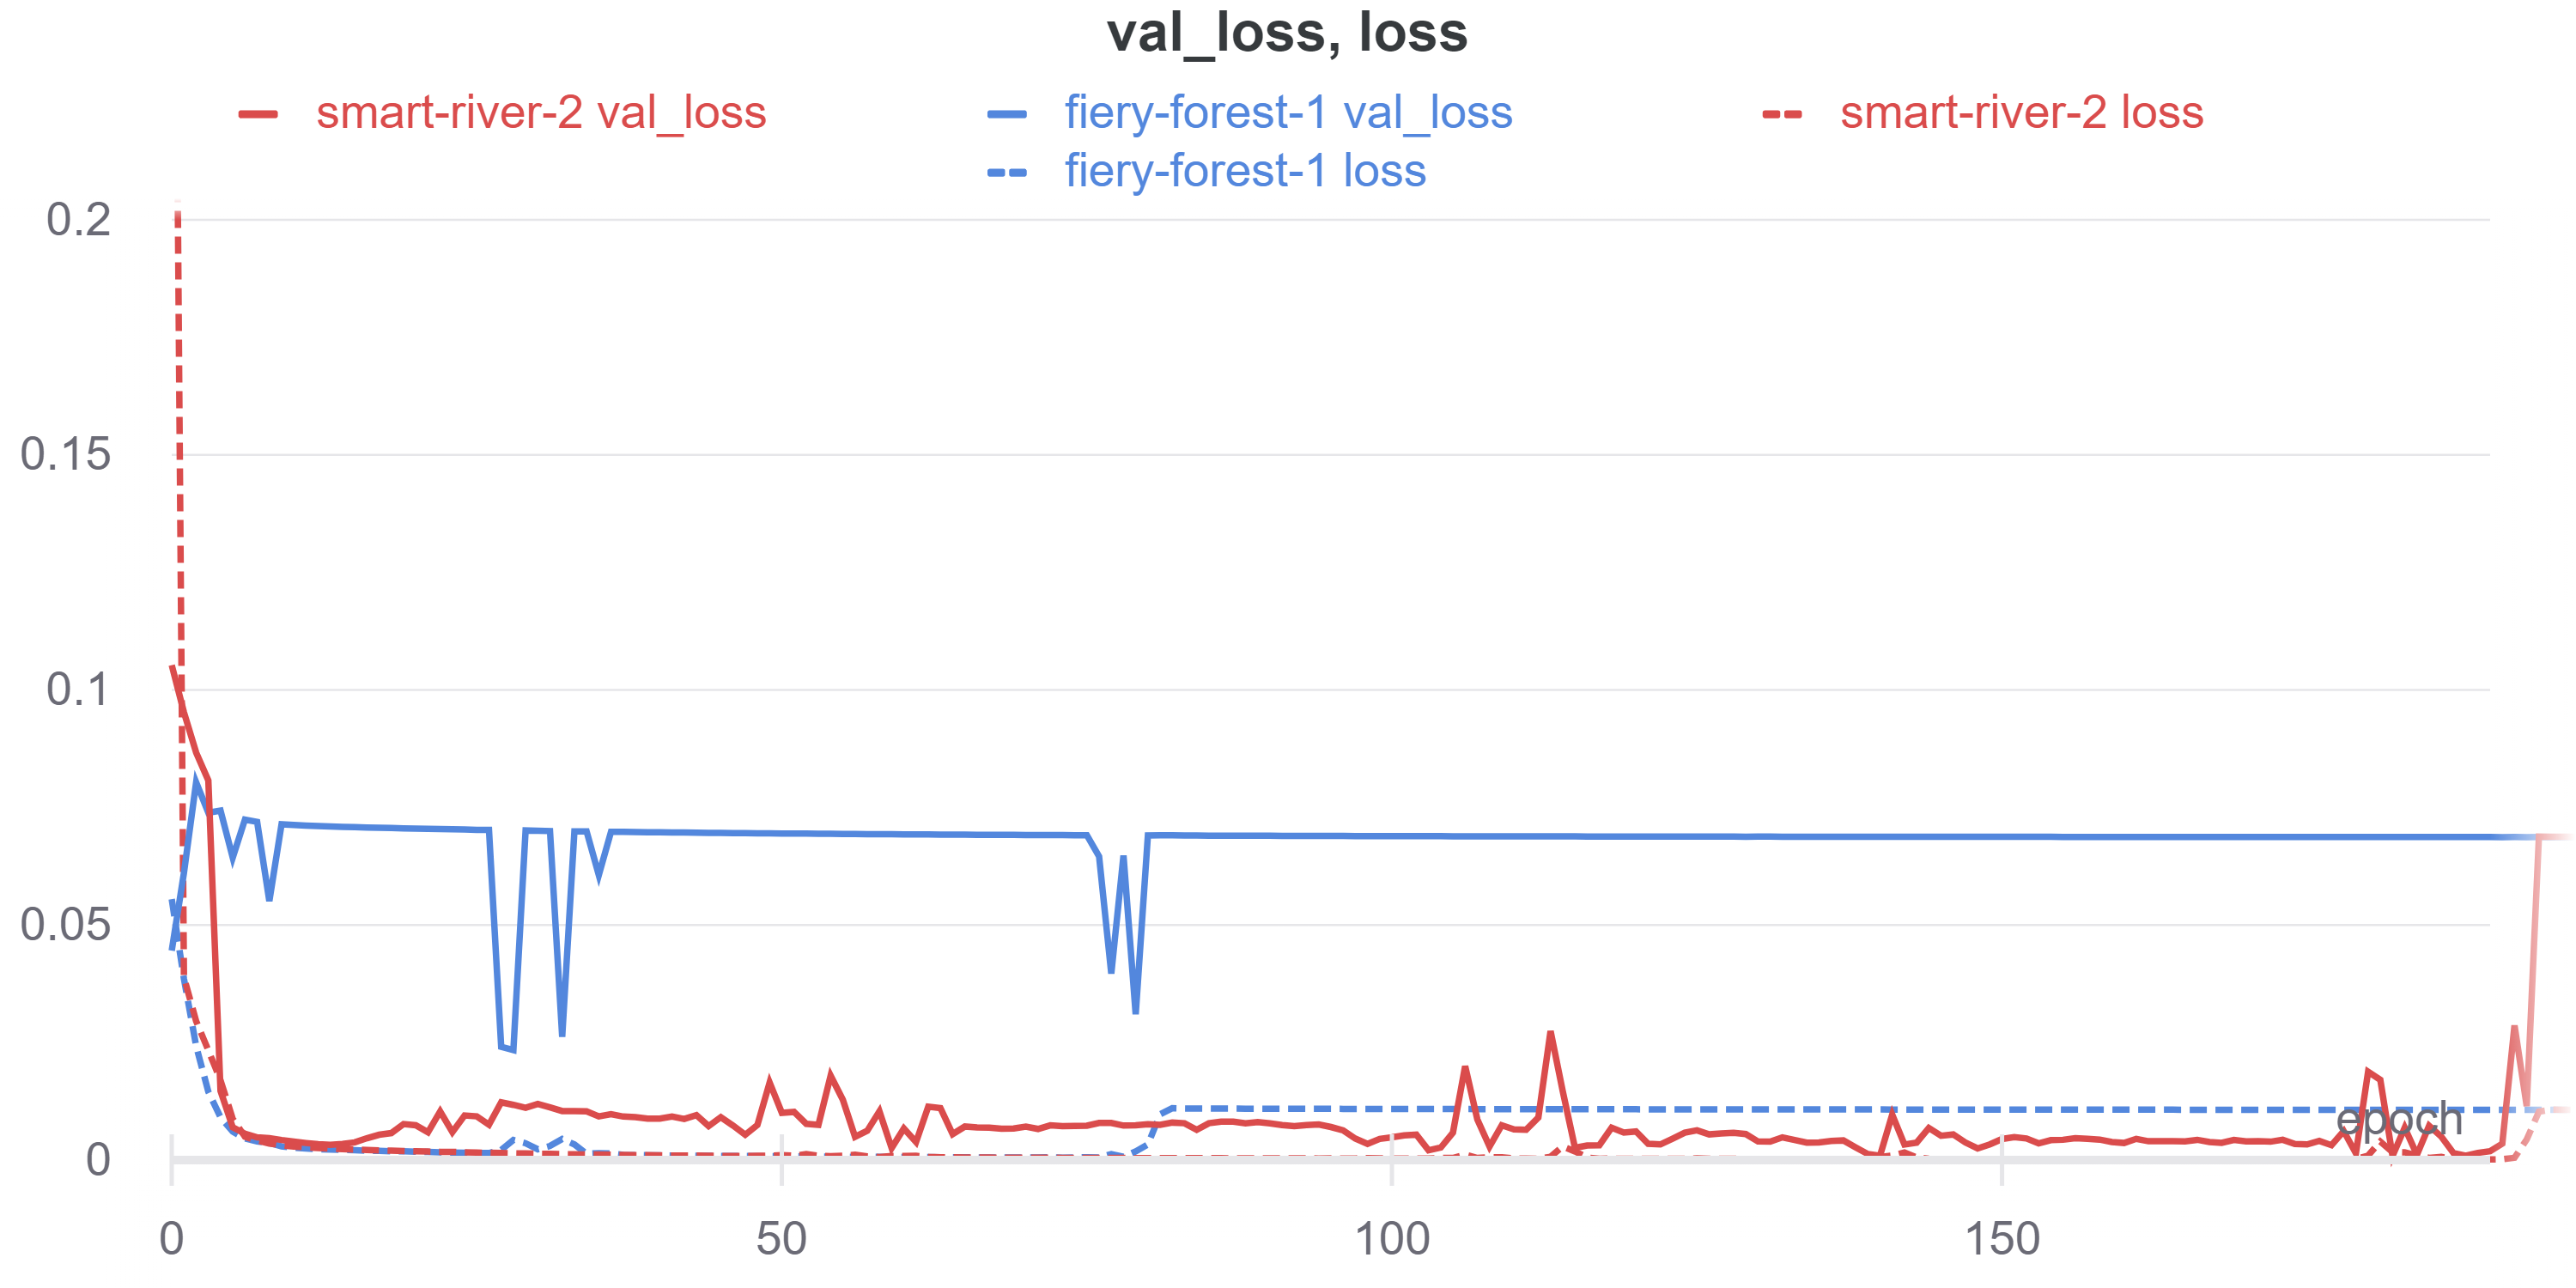
\includegraphics[width=\linewidth]{Chapters/Figures/best-params-meta1.png}
    \label{fig:meta-1-best}
    \caption[Hyperpamater Sweep 2]{Both iterations of the training process were run with identical network architectures and hyperparameters; however, the two runs have significantly different validation losses. The discrepancy is due to the random weights initialization process. We mitigate this problem by setting global random seeds throughout the training process to select consistent pseudo-random values. The slight difference in initial parameters causes one iteration to become "stuck" in a different local minimum, which performed similarly with the training set but made substantially worse predictions on the validation set. The goal of the first stage of the transfer learning process is to identify hyperparmaters which will lead to the best transfer learning candidates.}
\end{figure}

